\documentclass[11pt]{article}

    \usepackage[breakable]{tcolorbox}
    \usepackage{parskip} % Stop auto-indenting (to mimic markdown behaviour)
    

    % Basic figure setup, for now with no caption control since it's done
    % automatically by Pandoc (which extracts ![](path) syntax from Markdown).
    \usepackage{graphicx}
    % Maintain compatibility with old templates. Remove in nbconvert 6.0
    \let\Oldincludegraphics\includegraphics
    % Ensure that by default, figures have no caption (until we provide a
    % proper Figure object with a Caption API and a way to capture that
    % in the conversion process - todo).
    \usepackage{caption}
    \DeclareCaptionFormat{nocaption}{}
    \captionsetup{format=nocaption,aboveskip=0pt,belowskip=0pt}

    \usepackage{float}
    \floatplacement{figure}{H} % forces figures to be placed at the correct location
    \usepackage{xcolor} % Allow colors to be defined
    \usepackage{enumerate} % Needed for markdown enumerations to work
    \usepackage{geometry} % Used to adjust the document margins
    \usepackage{amsmath} % Equations
    \usepackage{amssymb} % Equations
    \usepackage{textcomp} % defines textquotesingle
    % Hack from http://tex.stackexchange.com/a/47451/13684:
    \AtBeginDocument{%
        \def\PYZsq{\textquotesingle}% Upright quotes in Pygmentized code
    }
    \usepackage{upquote} % Upright quotes for verbatim code
    \usepackage{eurosym} % defines \euro

    \usepackage{iftex}
    \ifPDFTeX
        \usepackage[T1]{fontenc}
        \IfFileExists{alphabeta.sty}{
              \usepackage{alphabeta}
          }{
              \usepackage[mathletters]{ucs}
              \usepackage[utf8x]{inputenc}
          }
    \else
        \usepackage{fontspec}
        \usepackage{unicode-math}
    \fi

    \usepackage{fancyvrb} % verbatim replacement that allows latex
    \usepackage{grffile} % extends the file name processing of package graphics
                         % to support a larger range
    \makeatletter % fix for old versions of grffile with XeLaTeX
    \@ifpackagelater{grffile}{2019/11/01}
    {
      % Do nothing on new versions
    }
    {
      \def\Gread@@xetex#1{%
        \IfFileExists{"\Gin@base".bb}%
        {\Gread@eps{\Gin@base.bb}}%
        {\Gread@@xetex@aux#1}%
      }
    }
    \makeatother
    \usepackage[Export]{adjustbox} % Used to constrain images to a maximum size
    \adjustboxset{max size={0.9\linewidth}{0.9\paperheight}}

    % The hyperref package gives us a pdf with properly built
    % internal navigation ('pdf bookmarks' for the table of contents,
    % internal cross-reference links, web links for URLs, etc.)
    \usepackage{hyperref}
    % The default LaTeX title has an obnoxious amount of whitespace. By default,
    % titling removes some of it. It also provides customization options.
    \usepackage{titling}
    \usepackage{longtable} % longtable support required by pandoc >1.10
    \usepackage{booktabs}  % table support for pandoc > 1.12.2
    \usepackage{array}     % table support for pandoc >= 2.11.3
    \usepackage{calc}      % table minipage width calculation for pandoc >= 2.11.1
    \usepackage[inline]{enumitem} % IRkernel/repr support (it uses the enumerate* environment)
    \usepackage[normalem]{ulem} % ulem is needed to support strikethroughs (\sout)
                                % normalem makes italics be italics, not underlines
    \usepackage{mathrsfs}
    

    
    % Colors for the hyperref package
    \definecolor{urlcolor}{rgb}{0,.145,.698}
    \definecolor{linkcolor}{rgb}{.71,0.21,0.01}
    \definecolor{citecolor}{rgb}{.12,.54,.11}

    % ANSI colors
    \definecolor{ansi-black}{HTML}{3E424D}
    \definecolor{ansi-black-intense}{HTML}{282C36}
    \definecolor{ansi-red}{HTML}{E75C58}
    \definecolor{ansi-red-intense}{HTML}{B22B31}
    \definecolor{ansi-green}{HTML}{00A250}
    \definecolor{ansi-green-intense}{HTML}{007427}
    \definecolor{ansi-yellow}{HTML}{DDB62B}
    \definecolor{ansi-yellow-intense}{HTML}{B27D12}
    \definecolor{ansi-blue}{HTML}{208FFB}
    \definecolor{ansi-blue-intense}{HTML}{0065CA}
    \definecolor{ansi-magenta}{HTML}{D160C4}
    \definecolor{ansi-magenta-intense}{HTML}{A03196}
    \definecolor{ansi-cyan}{HTML}{60C6C8}
    \definecolor{ansi-cyan-intense}{HTML}{258F8F}
    \definecolor{ansi-white}{HTML}{C5C1B4}
    \definecolor{ansi-white-intense}{HTML}{A1A6B2}
    \definecolor{ansi-default-inverse-fg}{HTML}{FFFFFF}
    \definecolor{ansi-default-inverse-bg}{HTML}{000000}

    % common color for the border for error outputs.
    \definecolor{outerrorbackground}{HTML}{FFDFDF}

    % commands and environments needed by pandoc snippets
    % extracted from the output of `pandoc -s`
    \providecommand{\tightlist}{%
      \setlength{\itemsep}{0pt}\setlength{\parskip}{0pt}}
    \DefineVerbatimEnvironment{Highlighting}{Verbatim}{commandchars=\\\{\}}
    % Add ',fontsize=\small' for more characters per line
    \newenvironment{Shaded}{}{}
    \newcommand{\KeywordTok}[1]{\textcolor[rgb]{0.00,0.44,0.13}{\textbf{{#1}}}}
    \newcommand{\DataTypeTok}[1]{\textcolor[rgb]{0.56,0.13,0.00}{{#1}}}
    \newcommand{\DecValTok}[1]{\textcolor[rgb]{0.25,0.63,0.44}{{#1}}}
    \newcommand{\BaseNTok}[1]{\textcolor[rgb]{0.25,0.63,0.44}{{#1}}}
    \newcommand{\FloatTok}[1]{\textcolor[rgb]{0.25,0.63,0.44}{{#1}}}
    \newcommand{\CharTok}[1]{\textcolor[rgb]{0.25,0.44,0.63}{{#1}}}
    \newcommand{\StringTok}[1]{\textcolor[rgb]{0.25,0.44,0.63}{{#1}}}
    \newcommand{\CommentTok}[1]{\textcolor[rgb]{0.38,0.63,0.69}{\textit{{#1}}}}
    \newcommand{\OtherTok}[1]{\textcolor[rgb]{0.00,0.44,0.13}{{#1}}}
    \newcommand{\AlertTok}[1]{\textcolor[rgb]{1.00,0.00,0.00}{\textbf{{#1}}}}
    \newcommand{\FunctionTok}[1]{\textcolor[rgb]{0.02,0.16,0.49}{{#1}}}
    \newcommand{\RegionMarkerTok}[1]{{#1}}
    \newcommand{\ErrorTok}[1]{\textcolor[rgb]{1.00,0.00,0.00}{\textbf{{#1}}}}
    \newcommand{\NormalTok}[1]{{#1}}

    % Additional commands for more recent versions of Pandoc
    \newcommand{\ConstantTok}[1]{\textcolor[rgb]{0.53,0.00,0.00}{{#1}}}
    \newcommand{\SpecialCharTok}[1]{\textcolor[rgb]{0.25,0.44,0.63}{{#1}}}
    \newcommand{\VerbatimStringTok}[1]{\textcolor[rgb]{0.25,0.44,0.63}{{#1}}}
    \newcommand{\SpecialStringTok}[1]{\textcolor[rgb]{0.73,0.40,0.53}{{#1}}}
    \newcommand{\ImportTok}[1]{{#1}}
    \newcommand{\DocumentationTok}[1]{\textcolor[rgb]{0.73,0.13,0.13}{\textit{{#1}}}}
    \newcommand{\AnnotationTok}[1]{\textcolor[rgb]{0.38,0.63,0.69}{\textbf{\textit{{#1}}}}}
    \newcommand{\CommentVarTok}[1]{\textcolor[rgb]{0.38,0.63,0.69}{\textbf{\textit{{#1}}}}}
    \newcommand{\VariableTok}[1]{\textcolor[rgb]{0.10,0.09,0.49}{{#1}}}
    \newcommand{\ControlFlowTok}[1]{\textcolor[rgb]{0.00,0.44,0.13}{\textbf{{#1}}}}
    \newcommand{\OperatorTok}[1]{\textcolor[rgb]{0.40,0.40,0.40}{{#1}}}
    \newcommand{\BuiltInTok}[1]{{#1}}
    \newcommand{\ExtensionTok}[1]{{#1}}
    \newcommand{\PreprocessorTok}[1]{\textcolor[rgb]{0.74,0.48,0.00}{{#1}}}
    \newcommand{\AttributeTok}[1]{\textcolor[rgb]{0.49,0.56,0.16}{{#1}}}
    \newcommand{\InformationTok}[1]{\textcolor[rgb]{0.38,0.63,0.69}{\textbf{\textit{{#1}}}}}
    \newcommand{\WarningTok}[1]{\textcolor[rgb]{0.38,0.63,0.69}{\textbf{\textit{{#1}}}}}


    % Define a nice break command that doesn't care if a line doesn't already
    % exist.
    \def\br{\hspace*{\fill} \\* }
    % Math Jax compatibility definitions
    \def\gt{>}
    \def\lt{<}
    \let\Oldtex\TeX
    \let\Oldlatex\LaTeX
    \renewcommand{\TeX}{\textrm{\Oldtex}}
    \renewcommand{\LaTeX}{\textrm{\Oldlatex}}
    % Document parameters
    % Document title
    \title{Relatório 6 Outubro}
    
    
    
    
    
% Pygments definitions
\makeatletter
\def\PY@reset{\let\PY@it=\relax \let\PY@bf=\relax%
    \let\PY@ul=\relax \let\PY@tc=\relax%
    \let\PY@bc=\relax \let\PY@ff=\relax}
\def\PY@tok#1{\csname PY@tok@#1\endcsname}
\def\PY@toks#1+{\ifx\relax#1\empty\else%
    \PY@tok{#1}\expandafter\PY@toks\fi}
\def\PY@do#1{\PY@bc{\PY@tc{\PY@ul{%
    \PY@it{\PY@bf{\PY@ff{#1}}}}}}}
\def\PY#1#2{\PY@reset\PY@toks#1+\relax+\PY@do{#2}}

\@namedef{PY@tok@w}{\def\PY@tc##1{\textcolor[rgb]{0.73,0.73,0.73}{##1}}}
\@namedef{PY@tok@c}{\let\PY@it=\textit\def\PY@tc##1{\textcolor[rgb]{0.24,0.48,0.48}{##1}}}
\@namedef{PY@tok@cp}{\def\PY@tc##1{\textcolor[rgb]{0.61,0.40,0.00}{##1}}}
\@namedef{PY@tok@k}{\let\PY@bf=\textbf\def\PY@tc##1{\textcolor[rgb]{0.00,0.50,0.00}{##1}}}
\@namedef{PY@tok@kp}{\def\PY@tc##1{\textcolor[rgb]{0.00,0.50,0.00}{##1}}}
\@namedef{PY@tok@kt}{\def\PY@tc##1{\textcolor[rgb]{0.69,0.00,0.25}{##1}}}
\@namedef{PY@tok@o}{\def\PY@tc##1{\textcolor[rgb]{0.40,0.40,0.40}{##1}}}
\@namedef{PY@tok@ow}{\let\PY@bf=\textbf\def\PY@tc##1{\textcolor[rgb]{0.67,0.13,1.00}{##1}}}
\@namedef{PY@tok@nb}{\def\PY@tc##1{\textcolor[rgb]{0.00,0.50,0.00}{##1}}}
\@namedef{PY@tok@nf}{\def\PY@tc##1{\textcolor[rgb]{0.00,0.00,1.00}{##1}}}
\@namedef{PY@tok@nc}{\let\PY@bf=\textbf\def\PY@tc##1{\textcolor[rgb]{0.00,0.00,1.00}{##1}}}
\@namedef{PY@tok@nn}{\let\PY@bf=\textbf\def\PY@tc##1{\textcolor[rgb]{0.00,0.00,1.00}{##1}}}
\@namedef{PY@tok@ne}{\let\PY@bf=\textbf\def\PY@tc##1{\textcolor[rgb]{0.80,0.25,0.22}{##1}}}
\@namedef{PY@tok@nv}{\def\PY@tc##1{\textcolor[rgb]{0.10,0.09,0.49}{##1}}}
\@namedef{PY@tok@no}{\def\PY@tc##1{\textcolor[rgb]{0.53,0.00,0.00}{##1}}}
\@namedef{PY@tok@nl}{\def\PY@tc##1{\textcolor[rgb]{0.46,0.46,0.00}{##1}}}
\@namedef{PY@tok@ni}{\let\PY@bf=\textbf\def\PY@tc##1{\textcolor[rgb]{0.44,0.44,0.44}{##1}}}
\@namedef{PY@tok@na}{\def\PY@tc##1{\textcolor[rgb]{0.41,0.47,0.13}{##1}}}
\@namedef{PY@tok@nt}{\let\PY@bf=\textbf\def\PY@tc##1{\textcolor[rgb]{0.00,0.50,0.00}{##1}}}
\@namedef{PY@tok@nd}{\def\PY@tc##1{\textcolor[rgb]{0.67,0.13,1.00}{##1}}}
\@namedef{PY@tok@s}{\def\PY@tc##1{\textcolor[rgb]{0.73,0.13,0.13}{##1}}}
\@namedef{PY@tok@sd}{\let\PY@it=\textit\def\PY@tc##1{\textcolor[rgb]{0.73,0.13,0.13}{##1}}}
\@namedef{PY@tok@si}{\let\PY@bf=\textbf\def\PY@tc##1{\textcolor[rgb]{0.64,0.35,0.47}{##1}}}
\@namedef{PY@tok@se}{\let\PY@bf=\textbf\def\PY@tc##1{\textcolor[rgb]{0.67,0.36,0.12}{##1}}}
\@namedef{PY@tok@sr}{\def\PY@tc##1{\textcolor[rgb]{0.64,0.35,0.47}{##1}}}
\@namedef{PY@tok@ss}{\def\PY@tc##1{\textcolor[rgb]{0.10,0.09,0.49}{##1}}}
\@namedef{PY@tok@sx}{\def\PY@tc##1{\textcolor[rgb]{0.00,0.50,0.00}{##1}}}
\@namedef{PY@tok@m}{\def\PY@tc##1{\textcolor[rgb]{0.40,0.40,0.40}{##1}}}
\@namedef{PY@tok@gh}{\let\PY@bf=\textbf\def\PY@tc##1{\textcolor[rgb]{0.00,0.00,0.50}{##1}}}
\@namedef{PY@tok@gu}{\let\PY@bf=\textbf\def\PY@tc##1{\textcolor[rgb]{0.50,0.00,0.50}{##1}}}
\@namedef{PY@tok@gd}{\def\PY@tc##1{\textcolor[rgb]{0.63,0.00,0.00}{##1}}}
\@namedef{PY@tok@gi}{\def\PY@tc##1{\textcolor[rgb]{0.00,0.52,0.00}{##1}}}
\@namedef{PY@tok@gr}{\def\PY@tc##1{\textcolor[rgb]{0.89,0.00,0.00}{##1}}}
\@namedef{PY@tok@ge}{\let\PY@it=\textit}
\@namedef{PY@tok@gs}{\let\PY@bf=\textbf}
\@namedef{PY@tok@gp}{\let\PY@bf=\textbf\def\PY@tc##1{\textcolor[rgb]{0.00,0.00,0.50}{##1}}}
\@namedef{PY@tok@go}{\def\PY@tc##1{\textcolor[rgb]{0.44,0.44,0.44}{##1}}}
\@namedef{PY@tok@gt}{\def\PY@tc##1{\textcolor[rgb]{0.00,0.27,0.87}{##1}}}
\@namedef{PY@tok@err}{\def\PY@bc##1{{\setlength{\fboxsep}{\string -\fboxrule}\fcolorbox[rgb]{1.00,0.00,0.00}{1,1,1}{\strut ##1}}}}
\@namedef{PY@tok@kc}{\let\PY@bf=\textbf\def\PY@tc##1{\textcolor[rgb]{0.00,0.50,0.00}{##1}}}
\@namedef{PY@tok@kd}{\let\PY@bf=\textbf\def\PY@tc##1{\textcolor[rgb]{0.00,0.50,0.00}{##1}}}
\@namedef{PY@tok@kn}{\let\PY@bf=\textbf\def\PY@tc##1{\textcolor[rgb]{0.00,0.50,0.00}{##1}}}
\@namedef{PY@tok@kr}{\let\PY@bf=\textbf\def\PY@tc##1{\textcolor[rgb]{0.00,0.50,0.00}{##1}}}
\@namedef{PY@tok@bp}{\def\PY@tc##1{\textcolor[rgb]{0.00,0.50,0.00}{##1}}}
\@namedef{PY@tok@fm}{\def\PY@tc##1{\textcolor[rgb]{0.00,0.00,1.00}{##1}}}
\@namedef{PY@tok@vc}{\def\PY@tc##1{\textcolor[rgb]{0.10,0.09,0.49}{##1}}}
\@namedef{PY@tok@vg}{\def\PY@tc##1{\textcolor[rgb]{0.10,0.09,0.49}{##1}}}
\@namedef{PY@tok@vi}{\def\PY@tc##1{\textcolor[rgb]{0.10,0.09,0.49}{##1}}}
\@namedef{PY@tok@vm}{\def\PY@tc##1{\textcolor[rgb]{0.10,0.09,0.49}{##1}}}
\@namedef{PY@tok@sa}{\def\PY@tc##1{\textcolor[rgb]{0.73,0.13,0.13}{##1}}}
\@namedef{PY@tok@sb}{\def\PY@tc##1{\textcolor[rgb]{0.73,0.13,0.13}{##1}}}
\@namedef{PY@tok@sc}{\def\PY@tc##1{\textcolor[rgb]{0.73,0.13,0.13}{##1}}}
\@namedef{PY@tok@dl}{\def\PY@tc##1{\textcolor[rgb]{0.73,0.13,0.13}{##1}}}
\@namedef{PY@tok@s2}{\def\PY@tc##1{\textcolor[rgb]{0.73,0.13,0.13}{##1}}}
\@namedef{PY@tok@sh}{\def\PY@tc##1{\textcolor[rgb]{0.73,0.13,0.13}{##1}}}
\@namedef{PY@tok@s1}{\def\PY@tc##1{\textcolor[rgb]{0.73,0.13,0.13}{##1}}}
\@namedef{PY@tok@mb}{\def\PY@tc##1{\textcolor[rgb]{0.40,0.40,0.40}{##1}}}
\@namedef{PY@tok@mf}{\def\PY@tc##1{\textcolor[rgb]{0.40,0.40,0.40}{##1}}}
\@namedef{PY@tok@mh}{\def\PY@tc##1{\textcolor[rgb]{0.40,0.40,0.40}{##1}}}
\@namedef{PY@tok@mi}{\def\PY@tc##1{\textcolor[rgb]{0.40,0.40,0.40}{##1}}}
\@namedef{PY@tok@il}{\def\PY@tc##1{\textcolor[rgb]{0.40,0.40,0.40}{##1}}}
\@namedef{PY@tok@mo}{\def\PY@tc##1{\textcolor[rgb]{0.40,0.40,0.40}{##1}}}
\@namedef{PY@tok@ch}{\let\PY@it=\textit\def\PY@tc##1{\textcolor[rgb]{0.24,0.48,0.48}{##1}}}
\@namedef{PY@tok@cm}{\let\PY@it=\textit\def\PY@tc##1{\textcolor[rgb]{0.24,0.48,0.48}{##1}}}
\@namedef{PY@tok@cpf}{\let\PY@it=\textit\def\PY@tc##1{\textcolor[rgb]{0.24,0.48,0.48}{##1}}}
\@namedef{PY@tok@c1}{\let\PY@it=\textit\def\PY@tc##1{\textcolor[rgb]{0.24,0.48,0.48}{##1}}}
\@namedef{PY@tok@cs}{\let\PY@it=\textit\def\PY@tc##1{\textcolor[rgb]{0.24,0.48,0.48}{##1}}}

\def\PYZbs{\char`\\}
\def\PYZus{\char`\_}
\def\PYZob{\char`\{}
\def\PYZcb{\char`\}}
\def\PYZca{\char`\^}
\def\PYZam{\char`\&}
\def\PYZlt{\char`\<}
\def\PYZgt{\char`\>}
\def\PYZsh{\char`\#}
\def\PYZpc{\char`\%}
\def\PYZdl{\char`\$}
\def\PYZhy{\char`\-}
\def\PYZsq{\char`\'}
\def\PYZdq{\char`\"}
\def\PYZti{\char`\~}
% for compatibility with earlier versions
\def\PYZat{@}
\def\PYZlb{[}
\def\PYZrb{]}
\makeatother


    % For linebreaks inside Verbatim environment from package fancyvrb.
    \makeatletter
        \newbox\Wrappedcontinuationbox
        \newbox\Wrappedvisiblespacebox
        \newcommand*\Wrappedvisiblespace {\textcolor{red}{\textvisiblespace}}
        \newcommand*\Wrappedcontinuationsymbol {\textcolor{red}{\llap{\tiny$\m@th\hookrightarrow$}}}
        \newcommand*\Wrappedcontinuationindent {3ex }
        \newcommand*\Wrappedafterbreak {\kern\Wrappedcontinuationindent\copy\Wrappedcontinuationbox}
        % Take advantage of the already applied Pygments mark-up to insert
        % potential linebreaks for TeX processing.
        %        {, <, #, %, $, ' and ": go to next line.
        %        _, }, ^, &, >, - and ~: stay at end of broken line.
        % Use of \textquotesingle for straight quote.
        \newcommand*\Wrappedbreaksatspecials {%
            \def\PYGZus{\discretionary{\char`\_}{\Wrappedafterbreak}{\char`\_}}%
            \def\PYGZob{\discretionary{}{\Wrappedafterbreak\char`\{}{\char`\{}}%
            \def\PYGZcb{\discretionary{\char`\}}{\Wrappedafterbreak}{\char`\}}}%
            \def\PYGZca{\discretionary{\char`\^}{\Wrappedafterbreak}{\char`\^}}%
            \def\PYGZam{\discretionary{\char`\&}{\Wrappedafterbreak}{\char`\&}}%
            \def\PYGZlt{\discretionary{}{\Wrappedafterbreak\char`\<}{\char`\<}}%
            \def\PYGZgt{\discretionary{\char`\>}{\Wrappedafterbreak}{\char`\>}}%
            \def\PYGZsh{\discretionary{}{\Wrappedafterbreak\char`\#}{\char`\#}}%
            \def\PYGZpc{\discretionary{}{\Wrappedafterbreak\char`\%}{\char`\%}}%
            \def\PYGZdl{\discretionary{}{\Wrappedafterbreak\char`\$}{\char`\$}}%
            \def\PYGZhy{\discretionary{\char`\-}{\Wrappedafterbreak}{\char`\-}}%
            \def\PYGZsq{\discretionary{}{\Wrappedafterbreak\textquotesingle}{\textquotesingle}}%
            \def\PYGZdq{\discretionary{}{\Wrappedafterbreak\char`\"}{\char`\"}}%
            \def\PYGZti{\discretionary{\char`\~}{\Wrappedafterbreak}{\char`\~}}%
        }
        % Some characters . , ; ? ! / are not pygmentized.
        % This macro makes them "active" and they will insert potential linebreaks
        \newcommand*\Wrappedbreaksatpunct {%
            \lccode`\~`\.\lowercase{\def~}{\discretionary{\hbox{\char`\.}}{\Wrappedafterbreak}{\hbox{\char`\.}}}%
            \lccode`\~`\,\lowercase{\def~}{\discretionary{\hbox{\char`\,}}{\Wrappedafterbreak}{\hbox{\char`\,}}}%
            \lccode`\~`\;\lowercase{\def~}{\discretionary{\hbox{\char`\;}}{\Wrappedafterbreak}{\hbox{\char`\;}}}%
            \lccode`\~`\:\lowercase{\def~}{\discretionary{\hbox{\char`\:}}{\Wrappedafterbreak}{\hbox{\char`\:}}}%
            \lccode`\~`\?\lowercase{\def~}{\discretionary{\hbox{\char`\?}}{\Wrappedafterbreak}{\hbox{\char`\?}}}%
            \lccode`\~`\!\lowercase{\def~}{\discretionary{\hbox{\char`\!}}{\Wrappedafterbreak}{\hbox{\char`\!}}}%
            \lccode`\~`\/\lowercase{\def~}{\discretionary{\hbox{\char`\/}}{\Wrappedafterbreak}{\hbox{\char`\/}}}%
            \catcode`\.\active
            \catcode`\,\active
            \catcode`\;\active
            \catcode`\:\active
            \catcode`\?\active
            \catcode`\!\active
            \catcode`\/\active
            \lccode`\~`\~
        }
    \makeatother

    \let\OriginalVerbatim=\Verbatim
    \makeatletter
    \renewcommand{\Verbatim}[1][1]{%
        %\parskip\z@skip
        \sbox\Wrappedcontinuationbox {\Wrappedcontinuationsymbol}%
        \sbox\Wrappedvisiblespacebox {\FV@SetupFont\Wrappedvisiblespace}%
        \def\FancyVerbFormatLine ##1{\hsize\linewidth
            \vtop{\raggedright\hyphenpenalty\z@\exhyphenpenalty\z@
                \doublehyphendemerits\z@\finalhyphendemerits\z@
                \strut ##1\strut}%
        }%
        % If the linebreak is at a space, the latter will be displayed as visible
        % space at end of first line, and a continuation symbol starts next line.
        % Stretch/shrink are however usually zero for typewriter font.
        \def\FV@Space {%
            \nobreak\hskip\z@ plus\fontdimen3\font minus\fontdimen4\font
            \discretionary{\copy\Wrappedvisiblespacebox}{\Wrappedafterbreak}
            {\kern\fontdimen2\font}%
        }%

        % Allow breaks at special characters using \PYG... macros.
        \Wrappedbreaksatspecials
        % Breaks at punctuation characters . , ; ? ! and / need catcode=\active
        \OriginalVerbatim[#1,codes*=\Wrappedbreaksatpunct]%
    }
    \makeatother

    % Exact colors from NB
    \definecolor{incolor}{HTML}{303F9F}
    \definecolor{outcolor}{HTML}{D84315}
    \definecolor{cellborder}{HTML}{CFCFCF}
    \definecolor{cellbackground}{HTML}{F7F7F7}

    % prompt
    \makeatletter
    \newcommand{\boxspacing}{\kern\kvtcb@left@rule\kern\kvtcb@boxsep}
    \makeatother
    \newcommand{\prompt}[4]{
        {\ttfamily\llap{{\color{#2}[#3]:\hspace{3pt}#4}}\vspace{-\baselineskip}}
    }
    

    
    % Prevent overflowing lines due to hard-to-break entities
    \sloppy
    % Setup hyperref package
    \hypersetup{
      breaklinks=true,  % so long urls are correctly broken across lines
      colorlinks=true,
      urlcolor=urlcolor,
      linkcolor=linkcolor,
      citecolor=citecolor,
      }
    % Slightly bigger margins than the latex defaults
    
    \geometry{verbose,tmargin=1in,bmargin=1in,lmargin=1in,rmargin=1in}
    
    

\begin{document}
    
    \maketitle
    
    

    
    \hypertarget{erf-relatorio-6-out}{%
\section{ERF Relatorio 6 Out}\label{erf-relatorio-6-out}}

\begin{quote}
Martinho Figueiredo (up201506179)

José Pedro Cruz (up201504646)
\end{quote}

    \hypertarget{abstrato}{%
\subsection{Abstrato}\label{abstrato}}

Este trabalho serve como introdução ao \emph{software} \textbf{ADS},
para desenho e analise de sistemas de radiofrequência e microondas. Para
tal, iremos adaptar duas cargas a configuraçoes de linha diferentes,
utilizabdo a ferramenta \emph{Line Calc} para obter as dimensões fisicas
da \emph{microstrip line} implementada. Usamos ainda o diagrama de Smith
presente no programa para normalizar a carga da alinea 2. Obtivemos
resultados favoraveis, que demonstram um alargamento da banda afectada
em torno da frequência de funcionamento, com o acréscimo de secçoes de
linha, sugerindo que estas introduzem sempre alguns pequenos defeitos
que se acumulam.

\hypertarget{para-uma-secuxe7uxe3o-de-lambda4-com-r_l-200}{%
\subsection{\texorpdfstring{Para uma secção de \(\lambda/4\), com
\(R_L = 200\)}{Para uma secção de \textbackslash lambda/4, com R\_L = 200}}\label{para-uma-secuxe7uxe3o-de-lambda4-com-r_l-200}}

Para este caso, primeiro calculamos a impedancia caracteristica da
secçao de linha adaptada, \(Z_{line}\).

    \begin{tcolorbox}[breakable, size=fbox, boxrule=1pt, pad at break*=1mm,colback=cellbackground, colframe=cellborder]
\prompt{In}{incolor}{1}{\boxspacing}
\begin{Verbatim}[commandchars=\\\{\}]
\PY{k+kn}{import} \PY{n+nn}{numpy} \PY{k}{as} \PY{n+nn}{np}
\PY{k+kn}{from} \PY{n+nn}{IPython}\PY{n+nn}{.}\PY{n+nn}{display} \PY{k+kn}{import} \PY{n}{Markdown} \PY{k}{as} \PY{n}{md}
\PY{n}{c} \PY{o}{=} \PY{l+m+mf}{3e8} \PY{c+c1}{\PYZsh{}light speed}
\PY{n}{f} \PY{o}{=} \PY{l+m+mf}{2e9} \PY{c+c1}{\PYZsh{} 2GHz Operating frequency}
\PY{n}{output} \PY{o}{=} \PY{l+s+s2}{\PYZdq{}}\PY{l+s+s2}{\PYZdq{}}
\PY{n}{Z\PYZus{}0} \PY{o}{=} \PY{l+m+mi}{50} \PY{c+c1}{\PYZsh{}Characteristic impedance of line}
\PY{n}{R\PYZus{}L} \PY{o}{=} \PY{l+m+mi}{200} \PY{c+c1}{\PYZsh{}Load impedance}
\PY{n}{Z\PYZus{}line} \PY{o}{=} \PY{n}{np}\PY{o}{.}\PY{n}{sqrt}\PY{p}{(}\PY{n}{Z\PYZus{}0}\PY{o}{*}\PY{n}{R\PYZus{}L}\PY{p}{)}\PY{c+c1}{\PYZsh{}impedance od microstrip  line}
\PY{n}{e\PYZus{}r} \PY{o}{=} \PY{l+m+mf}{3.2} \PY{c+c1}{\PYZsh{}from guide}
\PY{n}{wavlen} \PY{o}{=} \PY{n}{c}\PY{o}{/}\PY{n}{f}
\PY{n}{output} \PY{o}{+}\PY{o}{=} \PY{l+s+sa}{f}\PY{l+s+s1}{\PYZsq{}}\PY{l+s+s1}{\PYZdl{}\PYZdl{}Z\PYZus{}0 = }\PY{l+s+si}{\PYZob{}}\PY{n}{Z\PYZus{}0}\PY{l+s+si}{\PYZcb{}}\PY{l+s+s1}{ }\PY{l+s+s1}{\PYZbs{}}\PY{l+s+s1}{Omega\PYZdl{}\PYZdl{}}\PY{l+s+se}{\PYZbs{}n}\PY{l+s+s1}{\PYZsq{}}
\PY{n}{output} \PY{o}{+}\PY{o}{=} \PY{l+s+sa}{f}\PY{l+s+s1}{\PYZsq{}}\PY{l+s+s1}{\PYZdl{}\PYZdl{}R\PYZus{}L = }\PY{l+s+si}{\PYZob{}}\PY{n}{R\PYZus{}L}\PY{l+s+si}{\PYZcb{}}\PY{l+s+s1}{ }\PY{l+s+s1}{\PYZbs{}}\PY{l+s+s1}{Omega\PYZdl{}\PYZdl{}}\PY{l+s+se}{\PYZbs{}n}\PY{l+s+s1}{\PYZsq{}}
\PY{n}{output} \PY{o}{+}\PY{o}{=} \PY{l+s+sa}{f}\PY{l+s+s1}{\PYZsq{}}\PY{l+s+s1}{\PYZdl{}\PYZdl{}Z\PYZus{}}\PY{l+s+se}{\PYZob{}\PYZob{}}\PY{l+s+s1}{line}\PY{l+s+se}{\PYZcb{}\PYZcb{}}\PY{l+s+s1}{ = }\PY{l+s+s1}{\PYZbs{}}\PY{l+s+s1}{sqrt}\PY{l+s+se}{\PYZob{}\PYZob{}}\PY{l+s+s1}{Z\PYZus{}}\PY{l+s+se}{\PYZob{}\PYZob{}}\PY{l+s+s1}{0}\PY{l+s+se}{\PYZcb{}\PYZcb{}}\PY{l+s+s1}{ }\PY{l+s+s1}{\PYZbs{}}\PY{l+s+s1}{cdot R\PYZus{}}\PY{l+s+se}{\PYZob{}\PYZob{}}\PY{l+s+s1}{L}\PY{l+s+se}{\PYZcb{}\PYZcb{}}\PY{l+s+se}{\PYZcb{}\PYZcb{}}\PY{l+s+s1}{= }\PY{l+s+si}{\PYZob{}}\PY{n}{Z\PYZus{}line}\PY{l+s+si}{:}\PY{l+s+s1}{.0f}\PY{l+s+si}{\PYZcb{}}\PY{l+s+s1}{\PYZbs{}}\PY{l+s+s1}{Omega\PYZdl{}\PYZdl{}}\PY{l+s+se}{\PYZbs{}n}\PY{l+s+s1}{\PYZsq{}}

\PY{n}{output} \PY{o}{+}\PY{o}{=} \PY{l+s+sa}{f}\PY{l+s+s1}{\PYZsq{}}\PY{l+s+s1}{\PYZdl{}\PYZdl{}}\PY{l+s+s1}{\PYZbs{}}\PY{l+s+s1}{lambda = }\PY{l+s+si}{\PYZob{}}\PY{n}{wavlen}\PY{l+s+si}{:}\PY{l+s+s1}{.3f}\PY{l+s+si}{\PYZcb{}}\PY{l+s+s1}{m\PYZdl{}\PYZdl{}}\PY{l+s+se}{\PYZbs{}n}\PY{l+s+s1}{\PYZsq{}}
\PY{n}{md}\PY{p}{(}\PY{n}{output}\PY{p}{)}
\end{Verbatim}
\end{tcolorbox}
 
            
\prompt{Out}{outcolor}{1}{}
    
    \[Z_0 = 50 \Omega\] \[R_L = 200 \Omega\]
\[Z_{line} = \sqrt{Z_{0} \cdot R_{L}}= 100\Omega\] \[\lambda = 0.150m\]

    

    Utilizando estes valores no \emph{Line Calc}, com \(E_{Eff} = 90º\)
(\(\lambda/4\) corresponde a \(\frac{360º}{4} = 90º\) ) e \$Z\_0 =
Z\_\{line\} = 100 \Omega \$ obtivemos:

    \begin{figure}
\centering
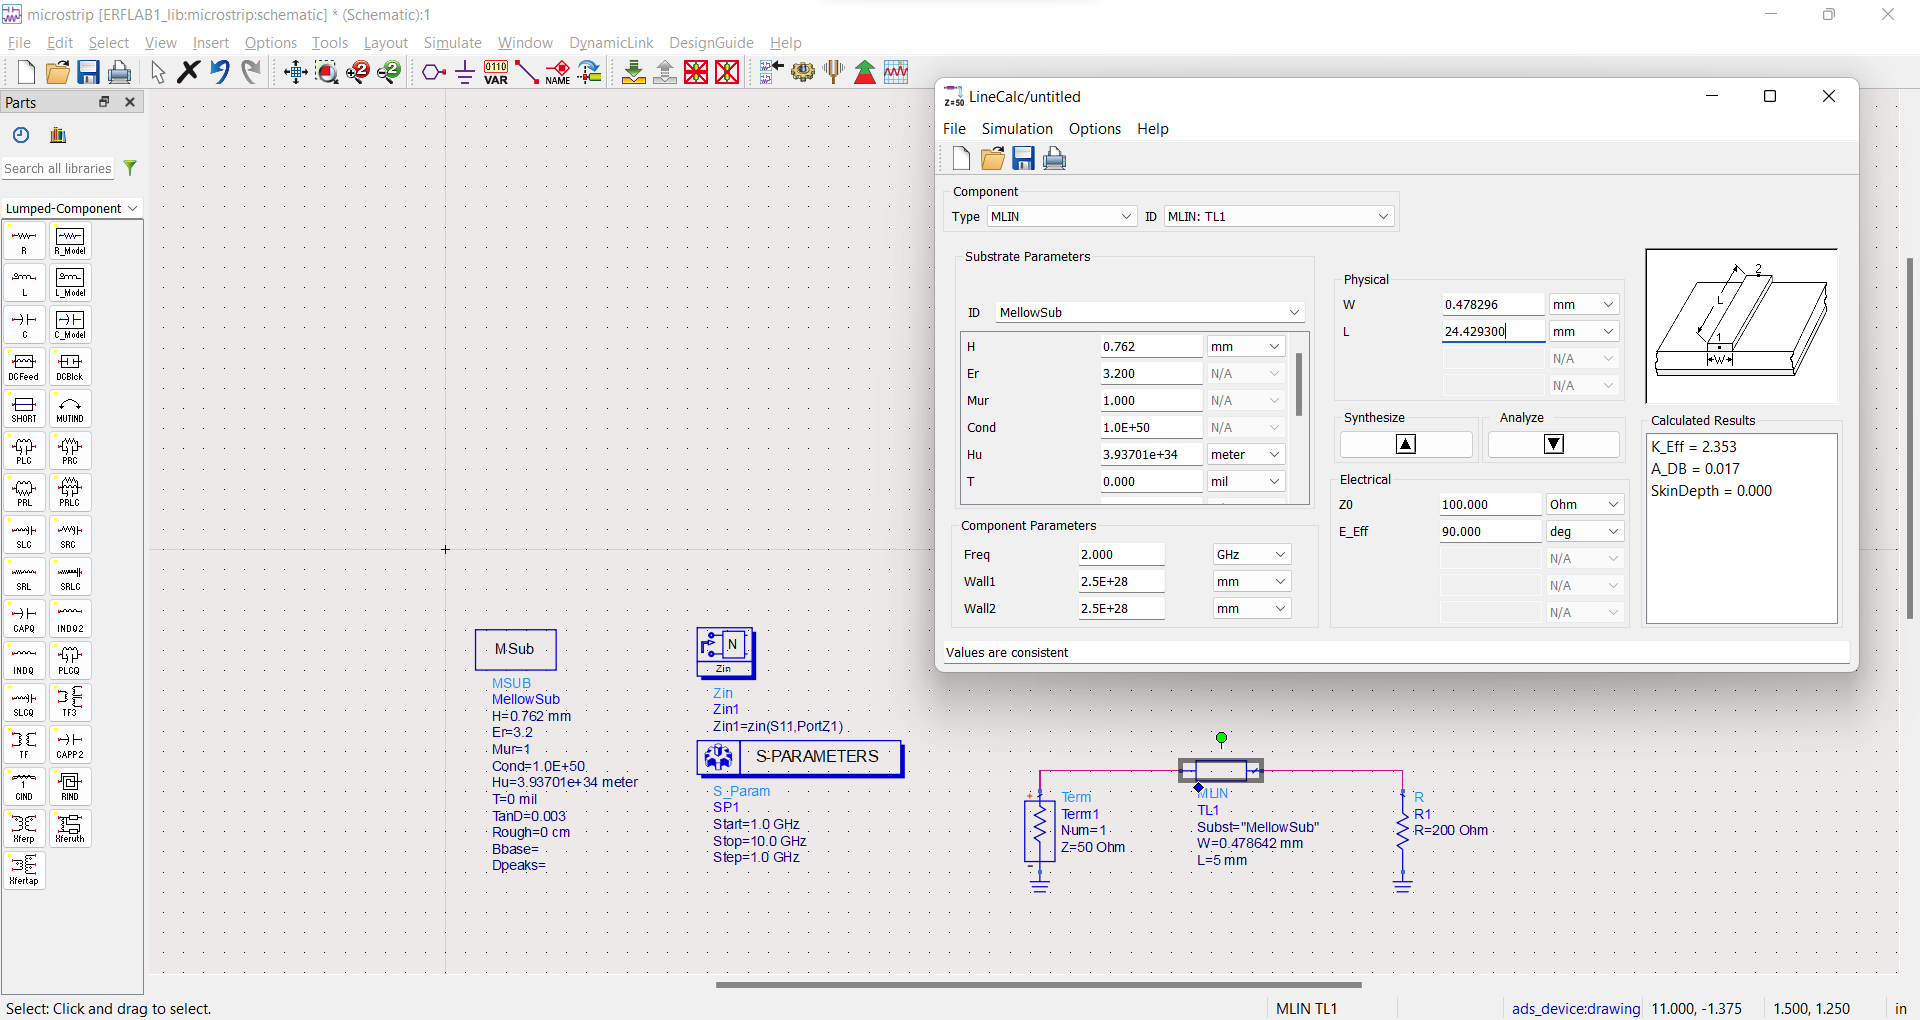
\includegraphics{media/1.0.png}
\caption{img1}
\end{figure}

    \begin{tcolorbox}[breakable, size=fbox, boxrule=1pt, pad at break*=1mm,colback=cellbackground, colframe=cellborder]
\prompt{In}{incolor}{2}{\boxspacing}
\begin{Verbatim}[commandchars=\\\{\}]
\PY{n}{output} \PY{o}{=} \PY{l+s+s2}{\PYZdq{}}\PY{l+s+s2}{\PYZdq{}}
\PY{c+c1}{\PYZsh{}FROM  ADS LINECALC}
\PY{c+c1}{\PYZsh{}\PYZhy{}\PYZhy{}\PYZhy{}\PYZhy{}\PYZhy{}}
\PY{n}{W} \PY{o}{=} \PY{l+m+mf}{0.478296e\PYZhy{}3} \PY{c+c1}{\PYZsh{}width }
\PY{n}{L} \PY{o}{=} \PY{l+m+mf}{24.4293e\PYZhy{}3} \PY{c+c1}{\PYZsh{}Lenght}
\PY{c+c1}{\PYZsh{}\PYZhy{}\PYZhy{}\PYZhy{}\PYZhy{}\PYZhy{}}
\PY{n}{K\PYZus{}eff} \PY{o}{=} \PY{l+m+mf}{2.53}
\PY{n}{A\PYZus{}DB} \PY{o}{=} \PY{l+m+mf}{0.017}
\PY{c+c1}{\PYZsh{}\PYZhy{}\PYZhy{}\PYZhy{}\PYZhy{}\PYZhy{}}
\PY{n}{output} \PY{o}{+}\PY{o}{=} \PY{l+s+sa}{f}\PY{l+s+s1}{\PYZsq{}}\PY{l+s+s1}{\PYZdl{}\PYZdl{}W = }\PY{l+s+si}{\PYZob{}}\PY{n}{W}\PY{l+s+si}{\PYZcb{}}\PY{l+s+s1}{ m\PYZdl{}\PYZdl{}}\PY{l+s+se}{\PYZbs{}n}\PY{l+s+s1}{\PYZsq{}}
\PY{n}{output} \PY{o}{+}\PY{o}{=} \PY{l+s+sa}{f}\PY{l+s+s1}{\PYZsq{}}\PY{l+s+s1}{\PYZdl{}\PYZdl{}L = }\PY{l+s+si}{\PYZob{}}\PY{n}{L}\PY{l+s+si}{\PYZcb{}}\PY{l+s+s1}{ m\PYZdl{}\PYZdl{}}\PY{l+s+se}{\PYZbs{}n}\PY{l+s+s1}{\PYZsq{}}
\PY{n}{md}\PY{p}{(}\PY{n}{output}\PY{p}{)}
\end{Verbatim}
\end{tcolorbox}
 
            
\prompt{Out}{outcolor}{2}{}
    
    \[W = 0.000478296 m\] \[L = 0.0244293 m\]

    

    \begin{tcolorbox}[breakable, size=fbox, boxrule=1pt, pad at break*=1mm,colback=cellbackground, colframe=cellborder]
\prompt{In}{incolor}{3}{\boxspacing}
\begin{Verbatim}[commandchars=\\\{\}]
\PY{c+c1}{\PYZsh{}Depth of the substrate}
\PY{n}{H} \PY{o}{=} \PY{l+m+mf}{0.762} \PY{c+c1}{\PYZsh{}from the guide}
\PY{c+c1}{\PYZsh{}Effective dielectric constant}
\PY{c+c1}{\PYZsh{}l =1e\PYZhy{}3 \PYZsh{}1mm should be changed to L from ads}
\PY{n}{e\PYZus{}ef} \PY{o}{=} \PY{p}{(}\PY{n}{e\PYZus{}r}\PY{o}{+}\PY{l+m+mi}{1}\PY{p}{)}\PY{o}{/}\PY{l+m+mi}{2}\PY{o}{+} \PY{p}{(}\PY{n}{e\PYZus{}r}\PY{o}{\PYZhy{}}\PY{l+m+mi}{1}\PY{p}{)}\PY{o}{/}\PY{l+m+mi}{2}\PY{o}{*}\PY{l+m+mi}{1}\PY{o}{/}\PY{n}{np}\PY{o}{.}\PY{n}{sqrt}\PY{p}{(}\PY{l+m+mi}{1}\PY{o}{+}\PY{l+m+mi}{12}\PY{o}{*}\PY{n}{H}\PY{o}{/}\PY{n}{W}\PY{p}{)}
\PY{n}{beta} \PY{o}{=} \PY{l+m+mi}{2}\PY{o}{*}\PY{n}{np}\PY{o}{.}\PY{n}{pi}\PY{o}{*}\PY{n}{f}\PY{o}{/}\PY{p}{(}\PY{n}{c}\PY{p}{)}\PY{o}{*}\PY{n}{np}\PY{o}{.}\PY{n}{sqrt}\PY{p}{(}\PY{n}{e\PYZus{}ef}\PY{p}{)}
\PY{n}{Z\PYZus{}in} \PY{o}{=} \PY{n}{Z\PYZus{}line}\PY{o}{*} \PY{p}{(}\PY{n}{R\PYZus{}L}\PY{o}{+}\PY{l+m+mi}{1}\PY{n}{j}\PY{o}{+}\PY{n}{Z\PYZus{}line}\PY{o}{*}\PY{n}{np}\PY{o}{.}\PY{n}{tan}\PY{p}{(}\PY{n}{beta}\PY{o}{*}\PY{n}{L}\PY{p}{)}\PY{p}{)}\PY{o}{/}\PY{p}{(}\PY{n}{Z\PYZus{}line}\PY{o}{+}\PY{l+m+mi}{1}\PY{n}{j}\PY{o}{*}\PY{n}{R\PYZus{}L}\PY{o}{*}\PY{n}{np}\PY{o}{.}\PY{n}{tan}\PY{p}{(}\PY{n}{beta}\PY{o}{*}\PY{n}{L}\PY{p}{)}\PY{p}{)}
\PY{n}{Gamma} \PY{o}{=} \PY{p}{(}\PY{n}{Z\PYZus{}in} \PY{o}{\PYZhy{}} \PY{n}{Z\PYZus{}0}\PY{p}{)}\PY{o}{/}\PY{p}{(}\PY{n}{Z\PYZus{}in} \PY{o}{+} \PY{n}{Z\PYZus{}0}\PY{p}{)}
\PY{n}{rho} \PY{o}{=} \PY{n}{np}\PY{o}{.}\PY{n}{abs}\PY{p}{(}\PY{n}{Gamma}\PY{p}{)}
\PY{n}{theta} \PY{o}{=} \PY{n}{np}\PY{o}{.}\PY{n}{angle}\PY{p}{(}\PY{n}{Gamma}\PY{p}{)}\PY{o}{*}\PY{l+m+mi}{180}\PY{o}{/}\PY{n}{np}\PY{o}{.}\PY{n}{pi}
\PY{n}{SwR} \PY{o}{=} \PY{p}{(}\PY{l+m+mi}{1} \PY{o}{+} \PY{n}{rho}\PY{p}{)}\PY{o}{/}\PY{p}{(}\PY{l+m+mi}{1} \PY{o}{\PYZhy{}} \PY{n}{rho}\PY{p}{)}


\PY{n}{output}\PY{o}{=}\PY{l+s+s1}{\PYZsq{}}\PY{l+s+s1}{\PYZsq{}}
\PY{n}{output}\PY{o}{+}\PY{o}{=}\PY{l+s+sa}{f}\PY{l+s+s1}{\PYZsq{}}\PY{l+s+s1}{\PYZdl{}\PYZdl{}E\PYZus{}}\PY{l+s+se}{\PYZob{}\PYZob{}}\PY{l+s+s1}{ef}\PY{l+s+se}{\PYZcb{}\PYZcb{}}\PY{l+s+s1}{ = }\PY{l+s+si}{\PYZob{}}\PY{n}{e\PYZus{}ef}\PY{l+s+si}{\PYZcb{}}\PY{l+s+s1}{\PYZdl{}\PYZdl{}}\PY{l+s+se}{\PYZbs{}n}\PY{l+s+s1}{\PYZsq{}}
\PY{n}{output}\PY{o}{+}\PY{o}{=}\PY{l+s+sa}{f}\PY{l+s+s1}{\PYZsq{}}\PY{l+s+s1}{\PYZdl{}\PYZdl{} B = }\PY{l+s+si}{\PYZob{}}\PY{n}{beta}\PY{l+s+si}{\PYZcb{}}\PY{l+s+s1}{\PYZdl{}\PYZdl{}}\PY{l+s+se}{\PYZbs{}n}\PY{l+s+s1}{\PYZsq{}}
\PY{n}{output}\PY{o}{+}\PY{o}{=}\PY{l+s+sa}{f}\PY{l+s+s1}{\PYZsq{}}\PY{l+s+s1}{\PYZdl{}\PYZdl{}Z\PYZus{}}\PY{l+s+se}{\PYZob{}\PYZob{}}\PY{l+s+s1}{in}\PY{l+s+se}{\PYZcb{}\PYZcb{}}\PY{l+s+s1}{= }\PY{l+s+si}{\PYZob{}}\PY{n}{Z\PYZus{}in}\PY{l+s+si}{\PYZcb{}}\PY{l+s+s1}{\PYZdl{}\PYZdl{}}\PY{l+s+se}{\PYZbs{}n}\PY{l+s+s1}{\PYZsq{}}
\PY{n}{output}\PY{o}{+}\PY{o}{=}\PY{l+s+sa}{f}\PY{l+s+s1}{\PYZsq{}}\PY{l+s+s1}{\PYZdl{}\PYZdl{}}\PY{l+s+s1}{\PYZbs{}}\PY{l+s+s1}{Gamma= }\PY{l+s+si}{\PYZob{}}\PY{n}{Gamma}\PY{l+s+si}{\PYZcb{}}\PY{l+s+s1}{\PYZdl{}\PYZdl{}}\PY{l+s+se}{\PYZbs{}n}\PY{l+s+s1}{\PYZsq{}}
\PY{n}{output}\PY{o}{+}\PY{o}{=}\PY{l+s+sa}{f}\PY{l+s+s1}{\PYZsq{}}\PY{l+s+s1}{\PYZdl{}\PYZdl{}}\PY{l+s+s1}{\PYZbs{}}\PY{l+s+s1}{Rho= }\PY{l+s+si}{\PYZob{}}\PY{n}{rho}\PY{l+s+si}{\PYZcb{}}\PY{l+s+s1}{\PYZdl{}\PYZdl{}}\PY{l+s+se}{\PYZbs{}n}\PY{l+s+s1}{\PYZsq{}}
\PY{n}{output}\PY{o}{+}\PY{o}{=}\PY{l+s+sa}{f}\PY{l+s+s1}{\PYZsq{}}\PY{l+s+s1}{\PYZdl{}\PYZdl{}}\PY{l+s+s1}{\PYZbs{}}\PY{l+s+s1}{Theta= }\PY{l+s+si}{\PYZob{}}\PY{n}{theta}\PY{l+s+si}{\PYZcb{}}\PY{l+s+s1}{\PYZdl{}\PYZdl{}}\PY{l+s+se}{\PYZbs{}n}\PY{l+s+s1}{\PYZsq{}}
\PY{n}{output}\PY{o}{+}\PY{o}{=}\PY{l+s+sa}{f}\PY{l+s+s1}{\PYZsq{}}\PY{l+s+s1}{\PYZdl{}\PYZdl{}SwR= }\PY{l+s+si}{\PYZob{}}\PY{n}{SwR}\PY{l+s+si}{\PYZcb{}}\PY{l+s+s1}{\PYZdl{}\PYZdl{}}\PY{l+s+se}{\PYZbs{}n}\PY{l+s+s1}{\PYZsq{}}
\PY{n}{md}\PY{p}{(}\PY{n}{output}\PY{p}{)}
\end{Verbatim}
\end{tcolorbox}
 
            
\prompt{Out}{outcolor}{3}{}
    
    \[E_{ef} = 2.1079553921574252\] \[ B = 60.816205173346454\]
\[Z_{in}= (2.534514689002848-58.4223992826539j)\]
\[\Gamma= (0.1489701539673856-0.9464102935128225j)\]
\[\Rho= 0.9580629157002651\] \[\Theta= -81.05472667076315\]
\[SwR= 46.69048762917084\]

    

    \begin{figure}
\centering
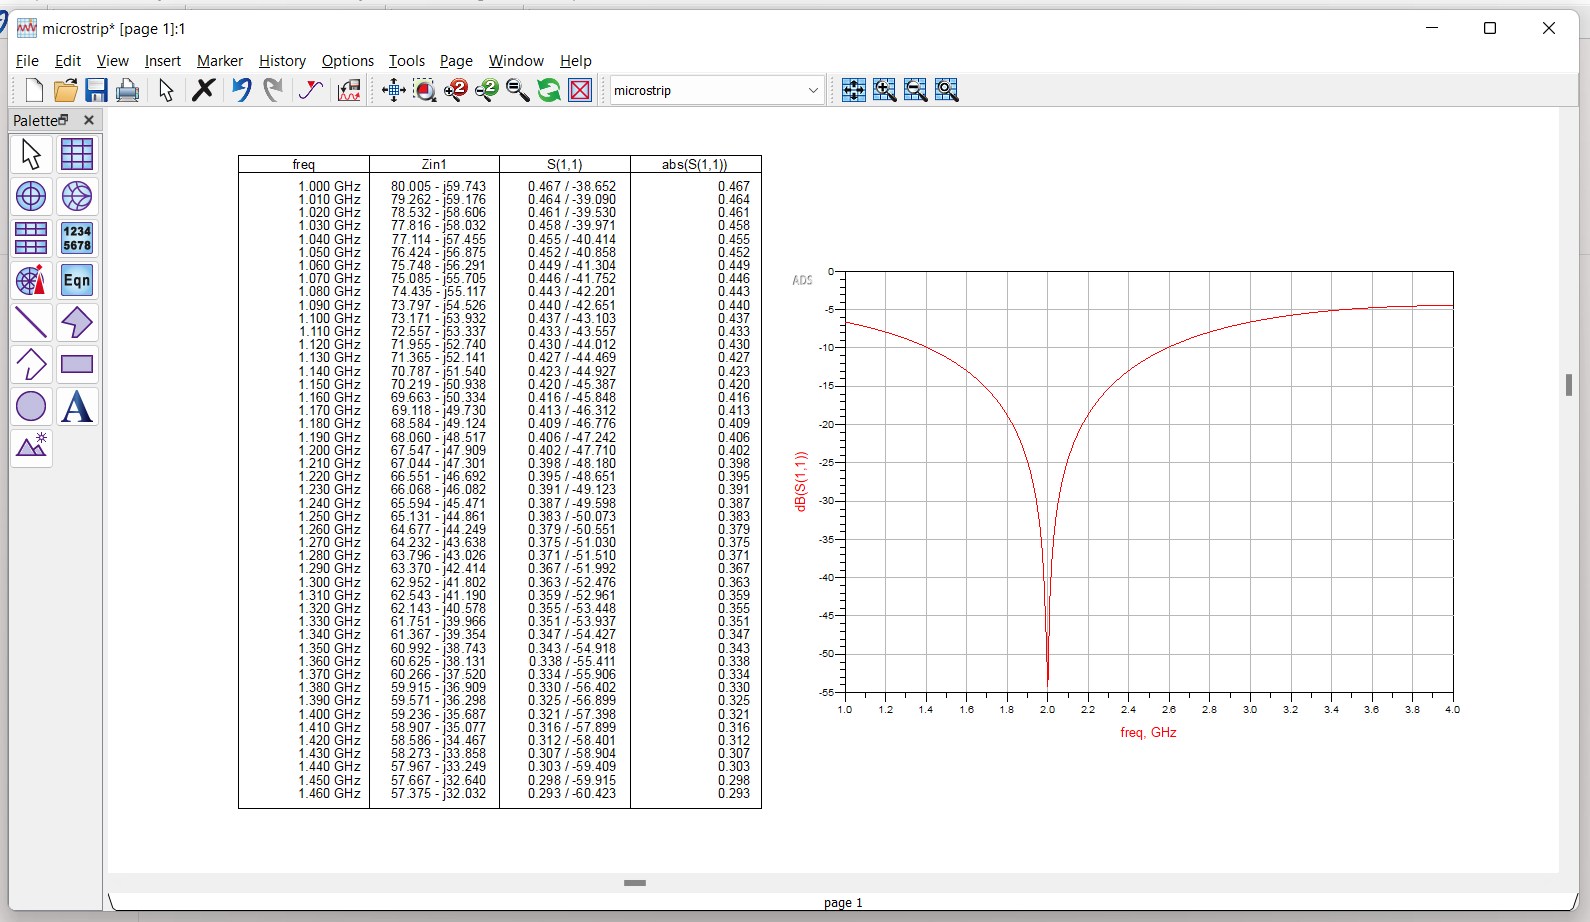
\includegraphics{media/1.1.png}
\caption{img2}
\end{figure}

    \hypertarget{para-3-secuxe7oes-de-linha-de-lambda4-de-comprimento}{%
\section{\texorpdfstring{Para 3 Secçoes de Linha de \(\lambda/4\) de
comprimento}{Para 3 Secçoes de Linha de \textbackslash lambda/4 de comprimento}}\label{para-3-secuxe7oes-de-linha-de-lambda4-de-comprimento}}

Utilizando a tabela da pag. 254 do livro ``Microwave Engineering'',
vemos que \(N=3\) porque temos 3 secções de linha.

    \begin{tcolorbox}[breakable, size=fbox, boxrule=1pt, pad at break*=1mm,colback=cellbackground, colframe=cellborder]
\prompt{In}{incolor}{4}{\boxspacing}
\begin{Verbatim}[commandchars=\\\{\}]
\PY{n}{output} \PY{o}{=} \PY{l+s+sa}{f}\PY{l+s+s1}{\PYZsq{}}\PY{l+s+s1}{\PYZdl{}\PYZdl{} R\PYZus{}}\PY{l+s+se}{\PYZob{}\PYZob{}}\PY{l+s+s1}{L}\PY{l+s+se}{\PYZcb{}\PYZcb{}}\PY{l+s+s1}{/}\PY{l+s+se}{\PYZob{}\PYZob{}}\PY{l+s+s1}{Z\PYZus{}0}\PY{l+s+se}{\PYZcb{}\PYZcb{}}\PY{l+s+s1}{ = }\PY{l+s+si}{\PYZob{}}\PY{n}{R\PYZus{}L}\PY{o}{/}\PY{n}{Z\PYZus{}0}\PY{l+s+si}{\PYZcb{}}\PY{l+s+s1}{\PYZdl{}\PYZdl{}}\PY{l+s+s1}{\PYZsq{}}
\PY{n}{md}\PY{p}{(}\PY{n}{output}\PY{p}{)}
\end{Verbatim}
\end{tcolorbox}
 
            
\prompt{Out}{outcolor}{4}{}
    
    \[ R_{L}/{Z_0} = 4.0\]

    

    Para \(N = 3\):

\begin{longtable}[]{@{}llll@{}}
\toprule
& \(\frac{Z_1}{Z_0}\) & \(\frac{Z_3}{Z_0}\) &
\(\frac{Z_3}{Z_0}\)\tabularnewline
\midrule
\endhead
\(\frac{R_L}{Z_0} = 4.0\) & 1.1907 & 2.0000 & 3.3594\tabularnewline
\bottomrule
\end{longtable}

    \begin{tcolorbox}[breakable, size=fbox, boxrule=1pt, pad at break*=1mm,colback=cellbackground, colframe=cellborder]
\prompt{In}{incolor}{5}{\boxspacing}
\begin{Verbatim}[commandchars=\\\{\}]
\PY{n}{Z\PYZus{}1} \PY{o}{=} \PY{l+m+mf}{1.1907} \PY{o}{*} \PY{n}{Z\PYZus{}0}
\PY{n}{Z\PYZus{}2} \PY{o}{=} \PY{l+m+mi}{2} \PY{o}{*} \PY{n}{Z\PYZus{}0}
\PY{n}{Z\PYZus{}3} \PY{o}{=} \PY{l+m+mf}{3.3594} \PY{o}{*} \PY{n}{Z\PYZus{}0}

\PY{n}{output}\PY{o}{=} \PY{l+s+s2}{\PYZdq{}}\PY{l+s+s2}{\PYZdq{}}
\PY{n}{output}\PY{o}{+}\PY{o}{=}\PY{l+s+sa}{f}\PY{l+s+s1}{\PYZsq{}}\PY{l+s+s1}{\PYZdl{}\PYZdl{}Z\PYZus{}1 = }\PY{l+s+si}{\PYZob{}}\PY{n}{Z\PYZus{}1}\PY{l+s+si}{\PYZcb{}}\PY{l+s+s1}{\PYZdl{}\PYZdl{}}\PY{l+s+se}{\PYZbs{}n}\PY{l+s+s1}{\PYZsq{}}
\PY{n}{output}\PY{o}{+}\PY{o}{=}\PY{l+s+sa}{f}\PY{l+s+s1}{\PYZsq{}}\PY{l+s+s1}{\PYZdl{}\PYZdl{}Z\PYZus{}2 = }\PY{l+s+si}{\PYZob{}}\PY{n}{Z\PYZus{}2}\PY{l+s+si}{\PYZcb{}}\PY{l+s+s1}{\PYZdl{}\PYZdl{}}\PY{l+s+se}{\PYZbs{}n}\PY{l+s+s1}{\PYZsq{}}
\PY{n}{output}\PY{o}{+}\PY{o}{=}\PY{l+s+sa}{f}\PY{l+s+s1}{\PYZsq{}}\PY{l+s+s1}{\PYZdl{}\PYZdl{}Z\PYZus{}3 = }\PY{l+s+si}{\PYZob{}}\PY{n}{Z\PYZus{}3}\PY{l+s+si}{\PYZcb{}}\PY{l+s+s1}{\PYZdl{}\PYZdl{}}\PY{l+s+se}{\PYZbs{}n}\PY{l+s+s1}{\PYZsq{}}

\PY{n}{md}\PY{p}{(}\PY{n}{output}\PY{p}{)}
\end{Verbatim}
\end{tcolorbox}
 
            
\prompt{Out}{outcolor}{5}{}
    
    \[Z_1 = 59.535000000000004\] \[Z_2 = 100\] \[Z_3 = 167.97\]

    

    Usando estes valores no \textbf{ADS} temos:

    \begin{figure}
\centering
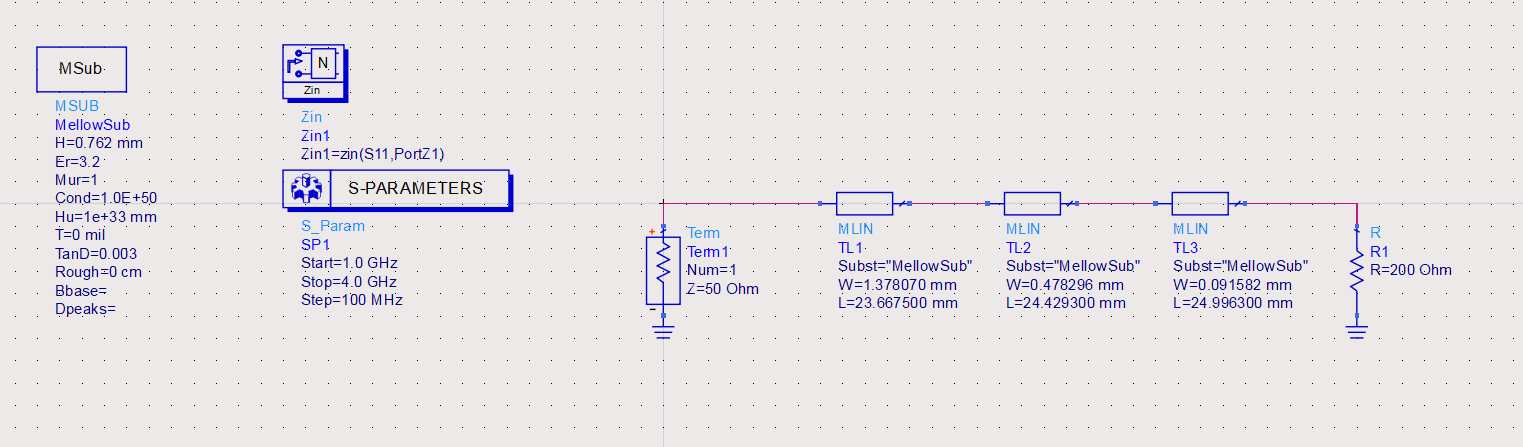
\includegraphics{media/2.0-corrigido.png}
\caption{img3}
\end{figure}

    \begin{figure}
\centering
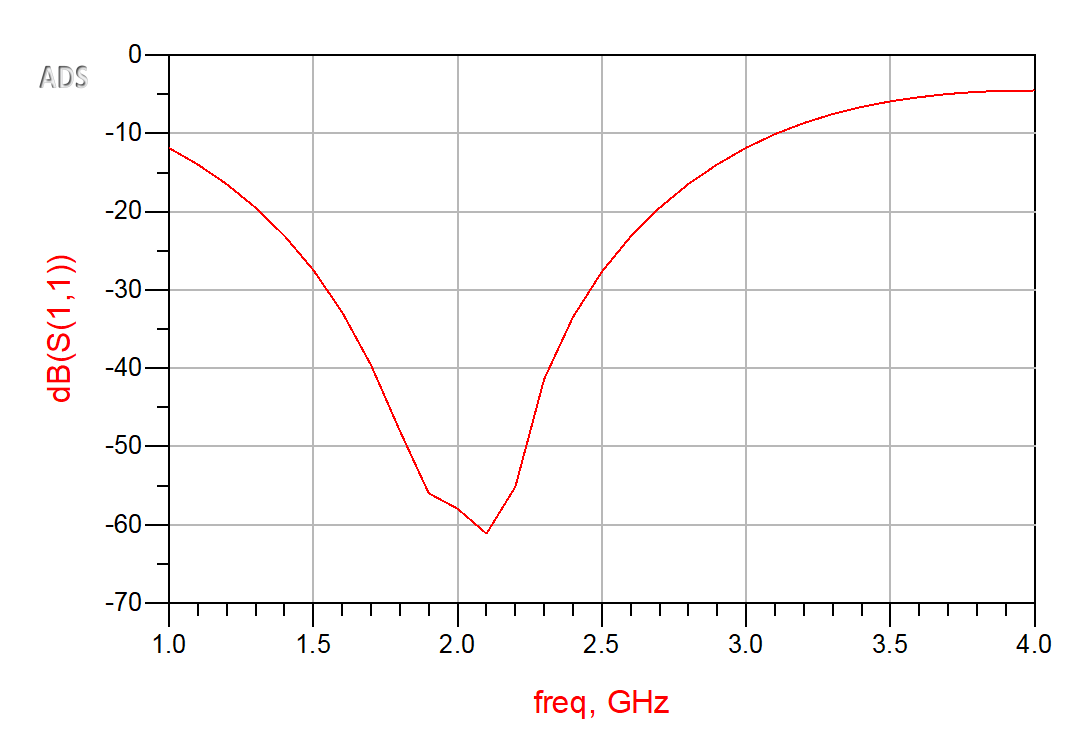
\includegraphics{media/2.1-corrigido.png}
\caption{img4}
\end{figure}

    \begin{figure}
\centering
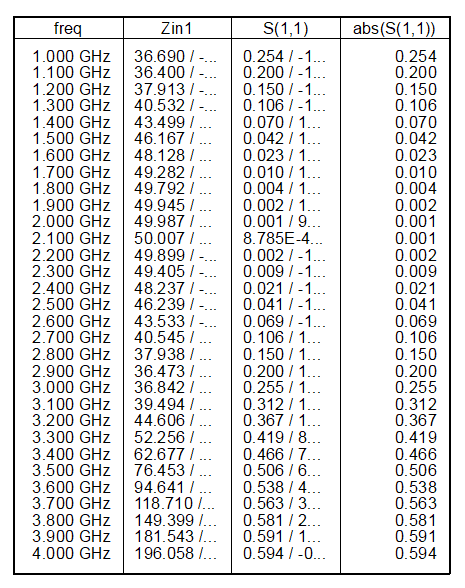
\includegraphics{media/2.2-corrigido.png}
\caption{img5}
\end{figure}

    \begin{figure}
\centering
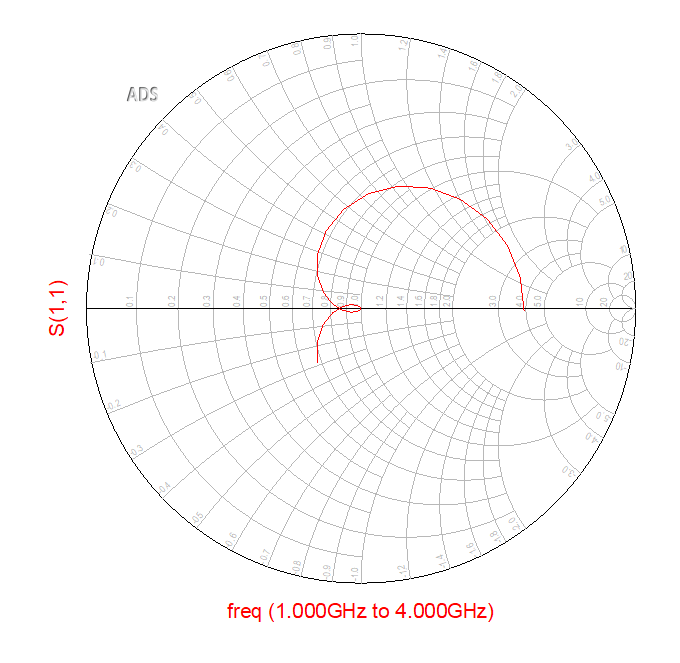
\includegraphics{media/2.3-corrigido.png}
\caption{img6}
\end{figure}

    \hypertarget{para-rl-10050j}{%
\subsection{Para RL = 100+50J}\label{para-rl-10050j}}

    \begin{tcolorbox}[breakable, size=fbox, boxrule=1pt, pad at break*=1mm,colback=cellbackground, colframe=cellborder]
\prompt{In}{incolor}{6}{\boxspacing}
\begin{Verbatim}[commandchars=\\\{\}]
\PY{n}{output} \PY{o}{=} \PY{l+s+s2}{\PYZdq{}}\PY{l+s+s2}{\PYZdq{}}
\PY{n}{Z\PYZus{}0} \PY{o}{=} \PY{l+m+mi}{50} \PY{c+c1}{\PYZsh{}Characteristic impedance of line}
\PY{n}{R\PYZus{}L} \PY{o}{=} \PY{l+m+mi}{100} \PY{o}{+} \PY{l+m+mi}{50}\PY{n}{j} \PY{c+c1}{\PYZsh{}Load impedance}
\PY{n}{Z\PYZus{}line} \PY{o}{=} \PY{n}{np}\PY{o}{.}\PY{n}{sqrt}\PY{p}{(}\PY{n}{Z\PYZus{}0}\PY{o}{*}\PY{n}{R\PYZus{}L}\PY{p}{)}\PY{c+c1}{\PYZsh{}impedance od microstrip  line}
\PY{n}{e\PYZus{}r} \PY{o}{=} \PY{l+m+mf}{3.2}
\PY{n}{wavlen} \PY{o}{=} \PY{n}{c}\PY{o}{/}\PY{n}{f}

\PY{n}{output} \PY{o}{+}\PY{o}{=} \PY{l+s+sa}{f}\PY{l+s+s1}{\PYZsq{}}\PY{l+s+s1}{\PYZdl{}\PYZdl{}Z\PYZus{}0 = }\PY{l+s+si}{\PYZob{}}\PY{n}{Z\PYZus{}0}\PY{l+s+si}{\PYZcb{}}\PY{l+s+s1}{ }\PY{l+s+s1}{\PYZbs{}}\PY{l+s+s1}{Omega\PYZdl{}\PYZdl{}}\PY{l+s+se}{\PYZbs{}n}\PY{l+s+s1}{\PYZsq{}}
\PY{n}{output} \PY{o}{+}\PY{o}{=} \PY{l+s+sa}{f}\PY{l+s+s1}{\PYZsq{}}\PY{l+s+s1}{\PYZdl{}\PYZdl{}R\PYZus{}L = }\PY{l+s+si}{\PYZob{}}\PY{n}{R\PYZus{}L}\PY{l+s+si}{\PYZcb{}}\PY{l+s+s1}{ }\PY{l+s+s1}{\PYZbs{}}\PY{l+s+s1}{Omega\PYZdl{}\PYZdl{}}\PY{l+s+se}{\PYZbs{}n}\PY{l+s+s1}{\PYZsq{}}
\PY{n}{output} \PY{o}{+}\PY{o}{=} \PY{l+s+sa}{f}\PY{l+s+s1}{\PYZsq{}}\PY{l+s+s1}{\PYZdl{}\PYZdl{}Z\PYZus{}}\PY{l+s+se}{\PYZob{}\PYZob{}}\PY{l+s+s1}{line}\PY{l+s+se}{\PYZcb{}\PYZcb{}}\PY{l+s+s1}{ = }\PY{l+s+s1}{\PYZbs{}}\PY{l+s+s1}{sqrt}\PY{l+s+se}{\PYZob{}\PYZob{}}\PY{l+s+s1}{Z\PYZus{}}\PY{l+s+se}{\PYZob{}\PYZob{}}\PY{l+s+s1}{0}\PY{l+s+se}{\PYZcb{}\PYZcb{}}\PY{l+s+s1}{ }\PY{l+s+s1}{\PYZbs{}}\PY{l+s+s1}{cdot R\PYZus{}}\PY{l+s+se}{\PYZob{}\PYZob{}}\PY{l+s+s1}{L}\PY{l+s+se}{\PYZcb{}\PYZcb{}}\PY{l+s+se}{\PYZcb{}\PYZcb{}}\PY{l+s+s1}{= }\PY{l+s+si}{\PYZob{}}\PY{n}{Z\PYZus{}line}\PY{l+s+si}{:}\PY{l+s+s1}{.0f}\PY{l+s+si}{\PYZcb{}}\PY{l+s+s1}{\PYZbs{}}\PY{l+s+s1}{Omega\PYZdl{}\PYZdl{}}\PY{l+s+se}{\PYZbs{}n}\PY{l+s+s1}{\PYZsq{}}

\PY{n}{output} \PY{o}{+}\PY{o}{=} \PY{l+s+sa}{f}\PY{l+s+s1}{\PYZsq{}}\PY{l+s+s1}{\PYZdl{}\PYZdl{}}\PY{l+s+s1}{\PYZbs{}}\PY{l+s+s1}{lambda = }\PY{l+s+si}{\PYZob{}}\PY{n}{wavlen}\PY{l+s+si}{:}\PY{l+s+s1}{.3f}\PY{l+s+si}{\PYZcb{}}\PY{l+s+s1}{m\PYZdl{}\PYZdl{}}\PY{l+s+se}{\PYZbs{}n}\PY{l+s+s1}{\PYZsq{}}
\PY{n}{md}\PY{p}{(}\PY{n}{output}\PY{p}{)}
\end{Verbatim}
\end{tcolorbox}
 
            
\prompt{Out}{outcolor}{6}{}
    
    \[Z_0 = 50 \Omega\] \[R_L = (100+50j) \Omega\]
\[Z_{line} = \sqrt{Z_{0} \cdot R_{L}}= 73+17j\Omega\]
\[\lambda = 0.150m\]

    


    % Add a bibliography block to the postdoc
    
    
    
\end{document}
